
\subsection{Implementation}
\label{sec:Implementation}

\paragraph{Patch size and stride.} In order to capture each frequency band at the right level of detail, I do not upsample the images $L_l(X)$ and use a small $3 \times 3$ patch size (with stride $1$). I experimented with larger patch sizes. However, this turned out to be counterproductive for the detail levelItarget, as details are blurred in larger patches. They also led to overfitting and were, in general, harder to optimise for. I used a stride of $1$, and hence patches overlap on the image plane. The overlapping patches are averaged while reconstructing the image.

\paragraph{Detail and colour modifications.} This work aims to capture intricate details present in highly detailed retouches and a wide range of image processing operators. Based on the observation that various operators can edit materials in the image space using the luminance component~\cite{Boyadzhiev15Band}, I focus on learning changes in luminance while preserving the input chrominance channels. 

\paragraph{Evaluation metrics.} To quantitatively compare the technique with state-of-the-art methods, I used PSNR and SSIM metrics. This is only possible if the before-after image pair was processed with a known, reproducible operator (see Section~\ref{sec:Comparisons} for details).


\paragraph{Training details.}\label{train_det} I train different mappings with the same structure, defined in Equation \ref{eq:weightedSum}, for each frequency band of the Laplacian pyramid. Each mapping consists of one MLP block and $K$ number of transformation matrices, which are learned jointly per frequency band from scratch for each before-after pair. The MLP block employed in the experiments consists of three fully-connected layers and non-linearities applied after each layer. The output size of the last layer is the same as the number of transformation matrices.

To normalize the weights, I choose the last activation function to be Softmax, while for the first two layers, I apply Leaky ReLU. Each transformation matrix is randomly initialised with the uniform distribution in the range of $[0, 1]$. All experiments use the Adam optimiser with a learning rate of $10^{-2}$, which exponentially decays with a decay rate of $0.96$. I use $l_1$ loss function in all experiments. Through backpropagation, both the MLP parameters and the entries of the transformation matrices are jointly learned. The pseudocode for both the training and inference procedures are the following:

\begin{algorithm}
\caption{One-shot Detail Retouching}
\SetKwFunction{FDetailRetouch}{Train}
\SetKwFunction{FPyramid}{LaplacianPyramid}
\SetKwFunction{FMLPBLOCK}{MLPBlock}
\SetKwFunction{FPatch}{ExtractPatch}
\SetKwFunction{Fprob}{Backpropagate}
\SetKwProg{Fn}{Function}{:}{}
\Fn{\FDetailRetouch{'before' image $X$, 'after' image $Y$}}{
	\Comment{Decompose images into its Laplacian bands.}\\
        $X_l \gets \FPyramid(X)$\;
        $Y_l \gets \FPyramid(Y)$\;
        
        \For{$l \gets 0$ \KwTo $n_l$}{
        \Comment{Extract patches from the images.}\\
        $x_i \gets \FPatch(X_l)$\;
        $y_i \gets \FPatch(Y_l)$\;
        $f_k \gets \FMLPBLOCK(x_i)$\;
        $y(x_i) \gets \sum^{K}_{k = 0} f_k(x_i) A_k x_i$\;
        $\mathcal{L} \gets E_{X, Y} \abs{(y(x_i) - y_i)}$\;  
        $(f_k, A_k) \gets \Fprob(\mathcal{L})$}
        }
\end{algorithm}

\begin{algorithm}
\caption{One-shot Detail Retouching}
\SetKwFunction{FDetailRetouch}{Inference}
\SetKwFunction{FPyramid}{LaplacianPyramid}
\SetKwFunction{FMLPBLOCK}{MLPBlock}
\SetKwFunction{FPatch}{ExtractPatch}
\SetKwFunction{Fpatchmerge}{MergePatch}
\SetKwProg{Fn}{Function}{:}{}
\Fn{\FDetailRetouch{input image $I$, blending weights $f_k$, transformation matrices $A_k$}}{

        $I_l \gets \FPyramid(I)$\;
        
        \For{$l \gets 0$ \KwTo $n_l$}{
        $i_i \gets \FPatch(I_l)$\;
        \Comment{Transform input patches $i_i$ with learned weights and matrices.}\\
        $o_i \gets \sum^{K}_{k = 1} f_k(i_i) A_k i_i$\;
        	\Comment{Place the patches on the output grid $O_l$.}\\
        $O_l \gets \Fpatchmerge(o_i)$}
     
        \Comment{Sum all output bands with input residual.}\\
        $O = I_{n_l} + \sum_l O_l$\;
        \Return $O$}
        
\end{algorithm}

\section{Results}
\label{sec:results}


\subsection{Ablation Studies}\label{ablation}
The success of the learned mappings relies on two key components: patch-adaptive retouching and transformation blending. I thus conduct experiments to illustrate the significance of these.

%Ifirst investigate the effect of the number of transformation matrices, $K$. 
% \paragraph*{Transformation Matrices.}
\paragraph{Transformation Matrices.} I compared transformation matrices of size $9 \times 9$ with scalar values. The method still remained spatially-varying, since I left the MLP the same, and used $K=256$ scalar weights. I tested both methods on 100 images and computed average PSNR values. I observed that the technique with matrices performed better than scalar values even in simple algorithmic filters, such as Gaussian and Unsharping Masking (around 2 dB and 3 dB higher PSNRs, respectively). 

As the complexity of a retouching style depends on multiple factors, such as artists’ design choices, user preferences, or the artist toolbox, it is challenging to analyse such effects on retouching examples quantitatively. For simple algorithmic filters, such as a Gaussian filter or unsharp masking, $K=1$ can sufficiently reproduce the filter. In contrast, more complex algorithms, such as a bilateral filter, require more matrices to capture the algorithmic edits accurately (Figure \ref{fig:ablation_K}). Since retouching edits combine the effect of multiple operators and are highly non-linear, I empirically found $K=256$ offers effective results for the retouching examples. 

\begin{figure}[th] % "[t!]" placement specifier just for this example
    \centering
	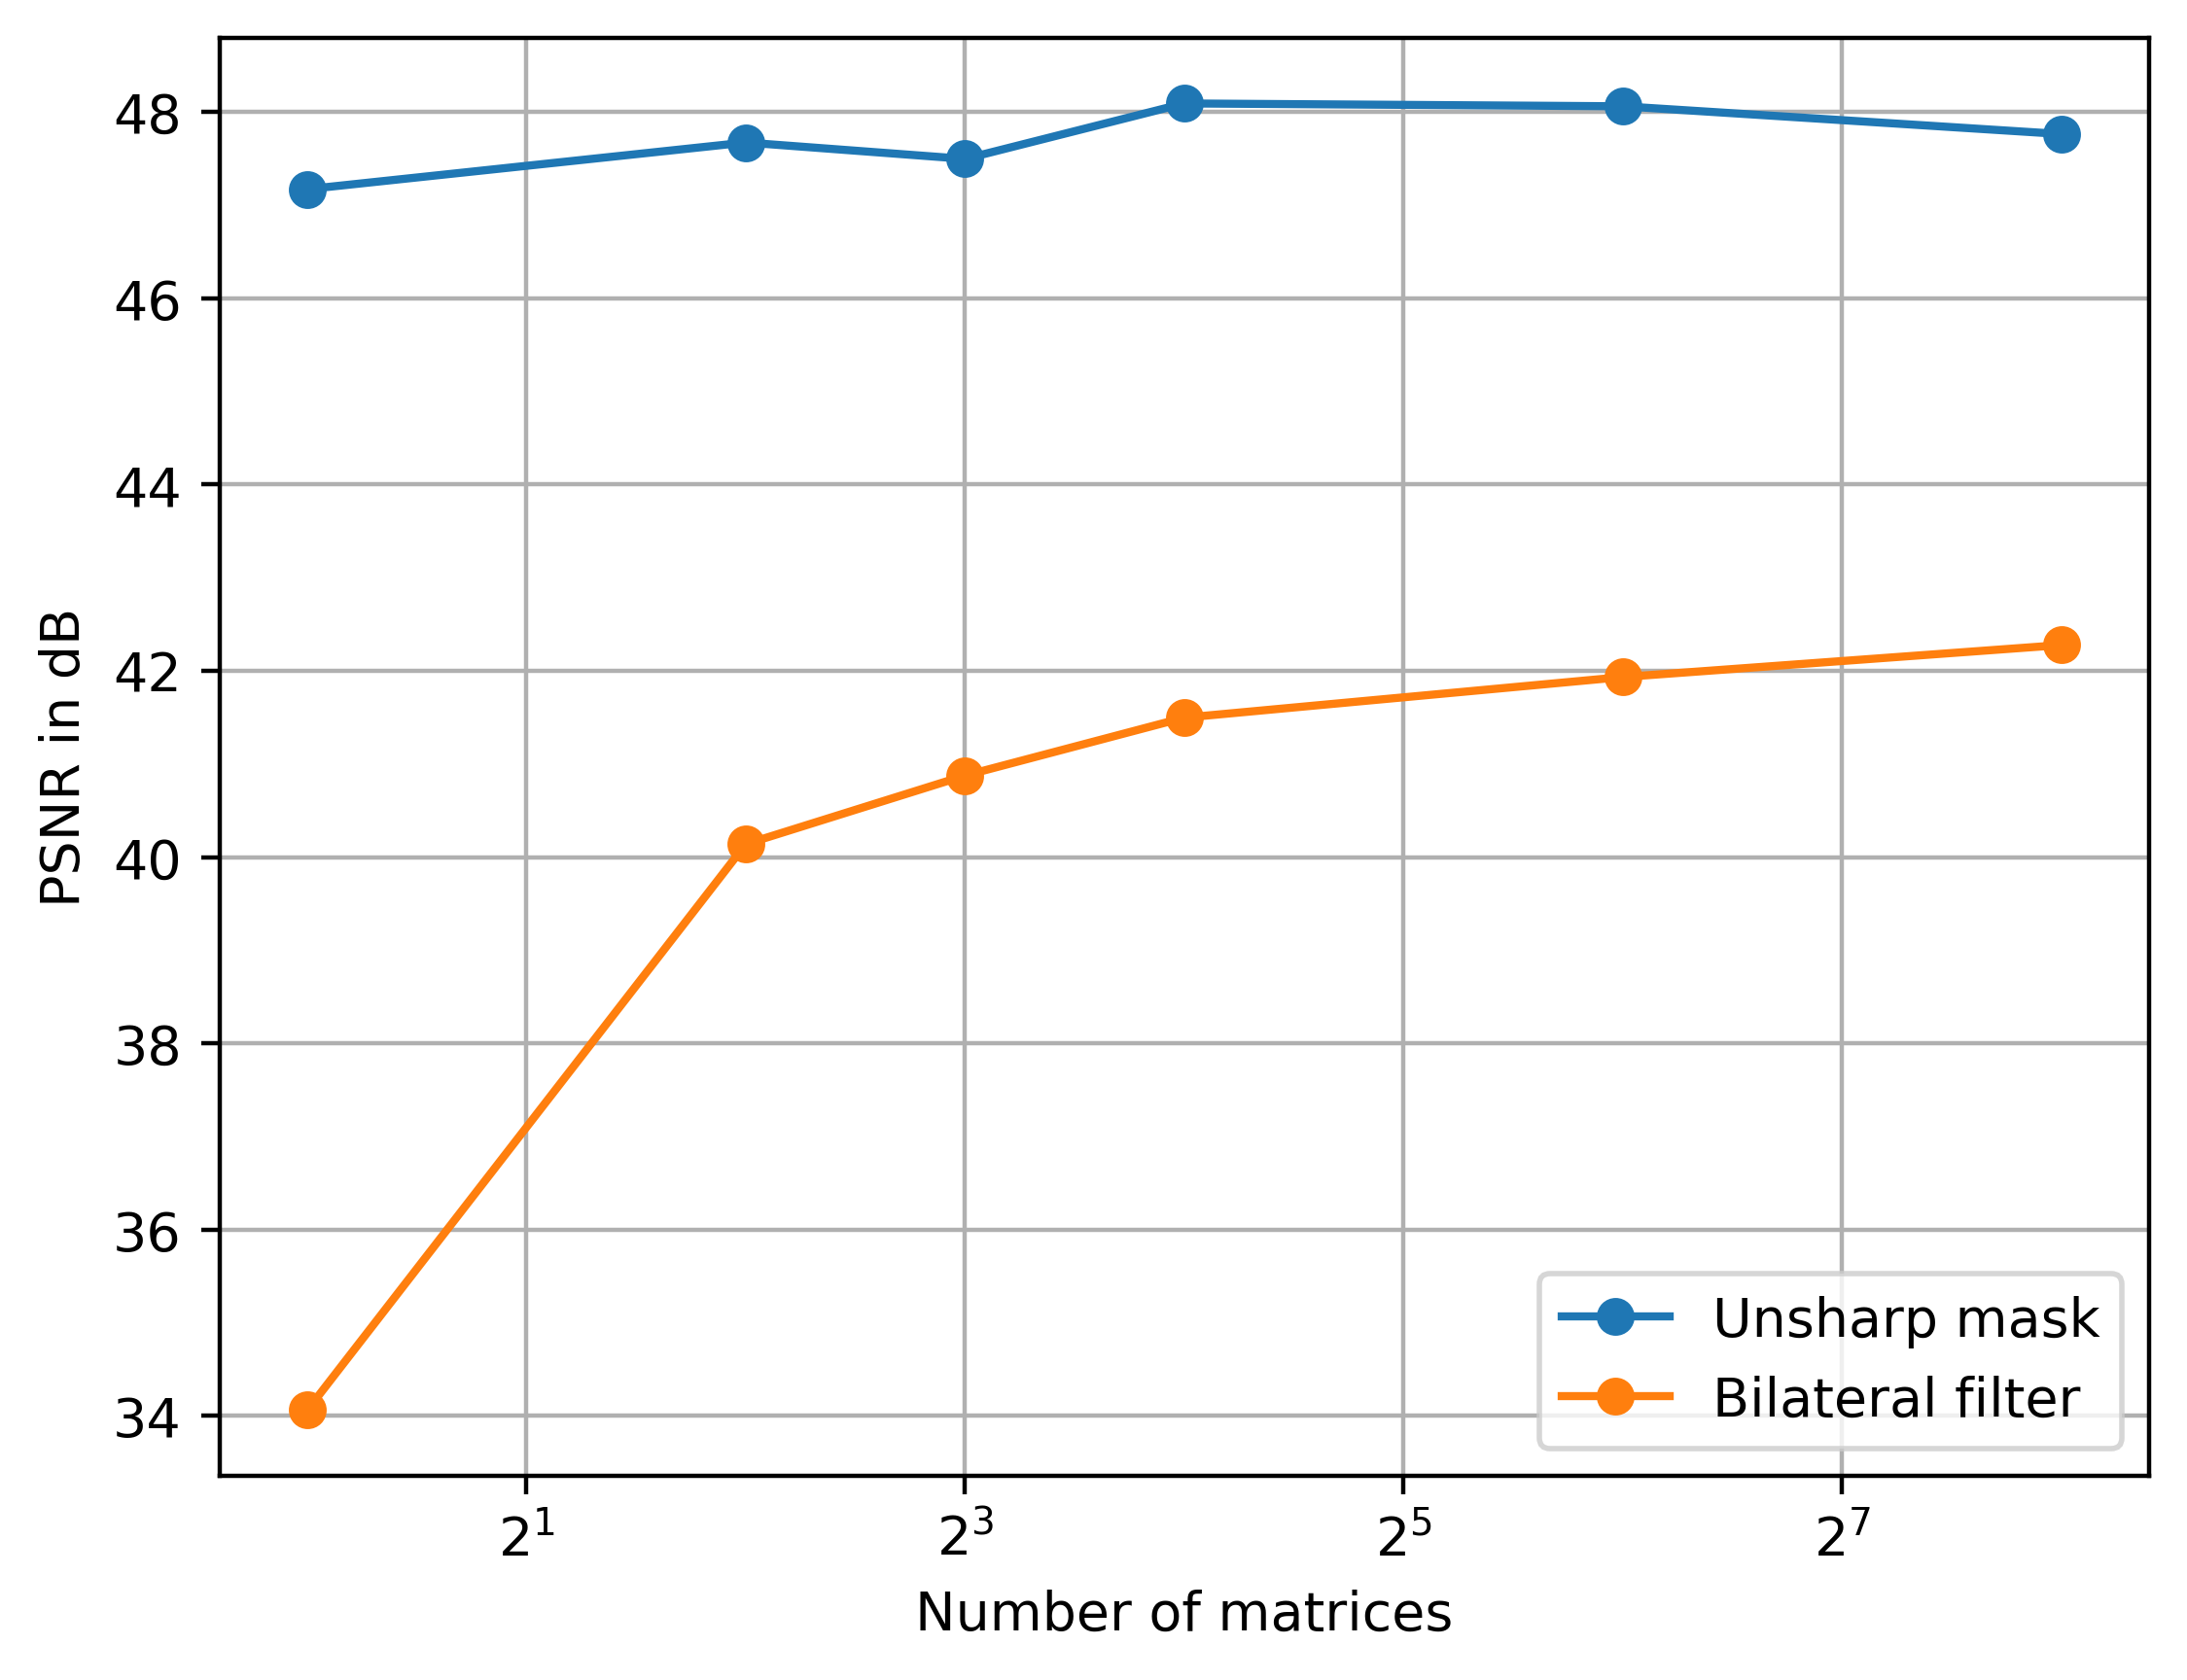
\includegraphics[width=0.5\columnwidth]{Chapters/detail-retouching-figs/ablation_matrices.png}

    \caption{The higher the complexity of the learned algorithm, the more transformation matrices the technique requires to capture the effects on local regions accurately. While $K=1$ can be sufficient for the model to capture unsharp masking, it requires more matrices to represent bilateral filtering precisely.}

    \label{fig:ablation_K}
\end{figure}

\begin{figure}%[H]
\centering
\includegraphics[width=0.8\columnwidth]{Chapters/detail-retouching-figs/AblationStudy_K.pdf}
    \caption{An MLP regressor cannot capture local edits, resulting in inaccurate retouching edits, such as blurring on the skin or around the eyes.}

\label{fig:ablation_MLP}
\end{figure}
% \paragraph*{Patch-adaptive Transformation Blending.}
\paragraph{Patch-adaptive Transformation Blending.} I also compared the patch-adaptive mapping to an MLP regressor on the extracted patches. This directly learns the mapping from the decomposition of example before-after images instead of utilising blended transformations. The MLP regressor follows a similar architecture as the MLP block (Figure \ref{fig:modelT}), with the only difference being the last activation function. I used Leaky ReLU here, since the Softmax function outputs pseudo-probabilities and is unsuitable for regression. Not explicitly handling the spatially-varying structure of the mapping and directly regressing limits the expressiveness of the model. This results in blurry results as shown in Figure~\ref{fig:ablation_MLP} because such a model cannot capture edits in intricate details, such as highlights around eyes and hair or brightening of the skin. I also tried increasing the capacity of the MLP regressor but did not observe much improvement in performance.


\paragraph{Weights visualisation.} To study the effectiveness of the weights across an image, I randomly chose eight transformation matrices and reconstructed their corresponding weights per Laplacian band. The reconstruction occurs in the same way as image patches, being placed in their location. However, since each patch of size $3 x 3$ has only one weight,Ido not need to take average over overlapping areas. Also, cropped the last eight columns of the reconstructed weight images since they were all zeros due to the size difference with patches. Figure \ref{fig:weight-vis} shows eight different reconstructed weights for each Laplacian band, obtained by the model trained with the example images in the teaser (middle \& right insets). The input to the model and the output retouched image are shown on top. As can be seen, the weights have varying values around different regions across the bands. Note that the resolution of the bands is increased to the same size for better visualisation. Otherwise, during training, each band’s resolution is kept its size based on the Laplacian pyramid.

\begin{figure}%[H]
\centering
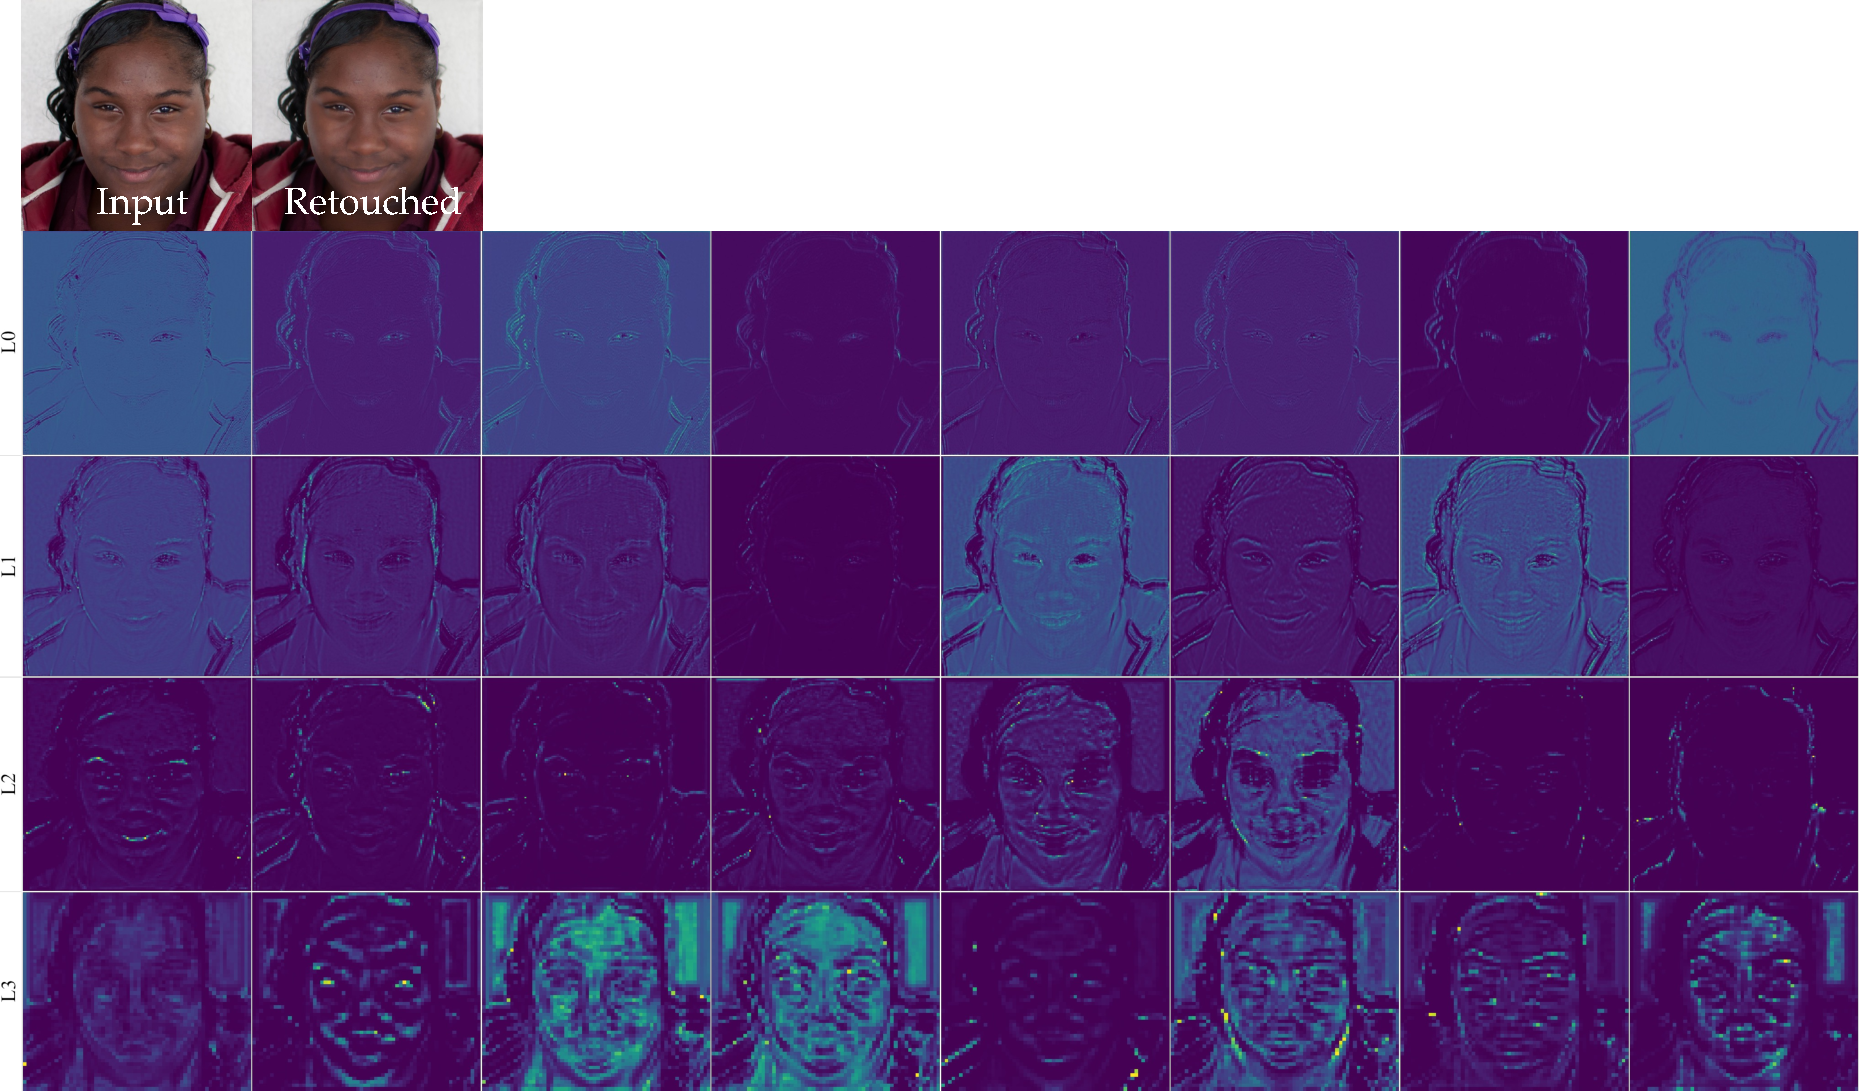
\includegraphics[width=0.8\columnwidth]{Chapters/detail-retouching-figs/weight_visualise.pdf}
    \caption{Visualisation of the reconstructed patch-adaptive weights of the model trained with example images in the teaser. Here, the input to the model is shown on top, and each row shows the weights in the corresponding Laplacian band, indicated on the left.}

\label{fig:weight-vis}
\end{figure}

\subsection{Qualitative Results}
I tested the proposed technique on a diverse range of before-after pairs, including face images from the \textbf{FFHQ} dataset \cite{karras2019style}.I focus on human portraits and face retouching in the experiments as they are arguably the most common and prioritised types of photos for retouching.I also illustrate that the technique provides visually pleasing results in different types of images, such as materials or rooms, and accurately captures image processing filters.

\begin{figure}[th] % "[t!]" placement specifier just for this example
    \centering
	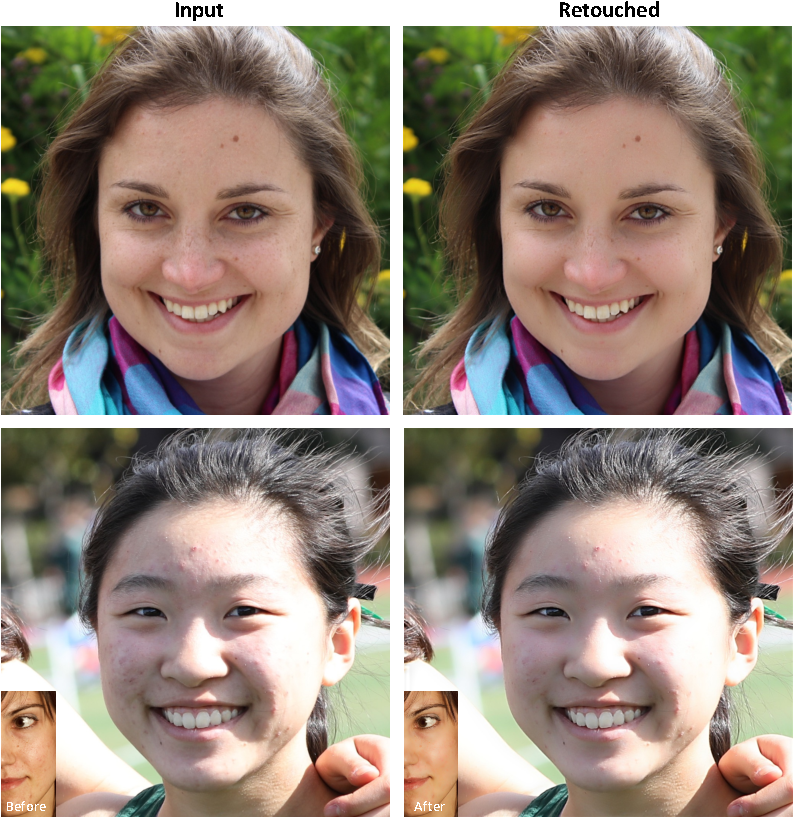
\includegraphics[width=0.8\columnwidth]{Chapters/detail-retouching-figs/res_diff_light_2_cvmp.pdf}
    \caption{\label{fig:newdataset_ex}The reproduced retouching style from the example pair (inset) improves skin texture without affecting fine details, such as eyes and hair, for a visually improved portrait. Moreover, the technique generalises well to faces with different lighting conditions and accurately reproduces the example retouching style.}
 
\end{figure}
% \paragraph*{Face retouching - skin and eye filters:}\label{faceretouching}
Human faces pose a particular challenge for the one-shot setting. However, the model can still capture highly nonlinear retouching edits and generalises well to different types of faces, view directions, and lighting conditions, as illustrated in Figures~\ref{fig:teaser}, ~\ref{fig:newdataset_ex}, and ~\ref{fig:retouchingstyles}.

\begin{figure}[th] % "[t!]" placement specifier just for this example
	\centering
	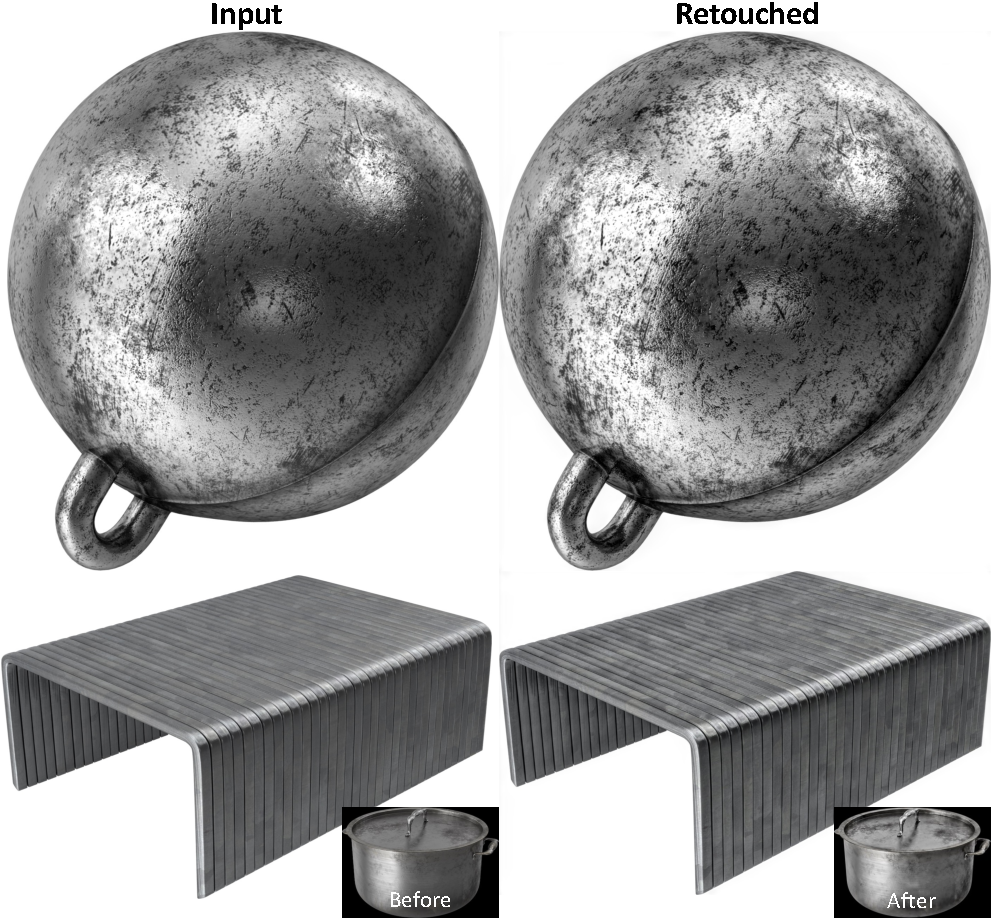
\includegraphics[width=0.8\columnwidth]{Chapters/detail-retouching-figs/MaterialResults.pdf}
    \caption{\label{fig:material_res}Material editing results on photos (left), and rendered images (right), based on the before-after pair (inset). The details, such as scratches or lines are emphasised, and materials became shinier. Image courtesy of royalmix (top and bottom-inset), tsmdunn (bottom). (PixelSquid).}

\end{figure}

The example pairs in Figures~\ref{fig:teaser}, ~\ref{fig:newdataset_ex}  and ~\ref{fig:retouchingstyles} were generated by brushing onto the skin with artist created brushes, eye sharpening (sharpening example in Figure~\ref{fig:teaser}), and further brightness/contrast adjustments. These brushes first decompose the skin into a detail and base layer, typically with frequency decomposition, alter the detail layer and blend it with the base layer. They differ in how (1) they decompose the skin into the layers, i.e., what frequencies are in each layer, and (2) they edit and blend each layer with different opacity values. This variation creates retouching nuances, as shown in Figure~\ref{fig:retouchingstyles}. The framework can still accurately capture such slight differences in styles. 

\begin{figure}[th] % "[t!]" placement specifier just for this example
    \centering
	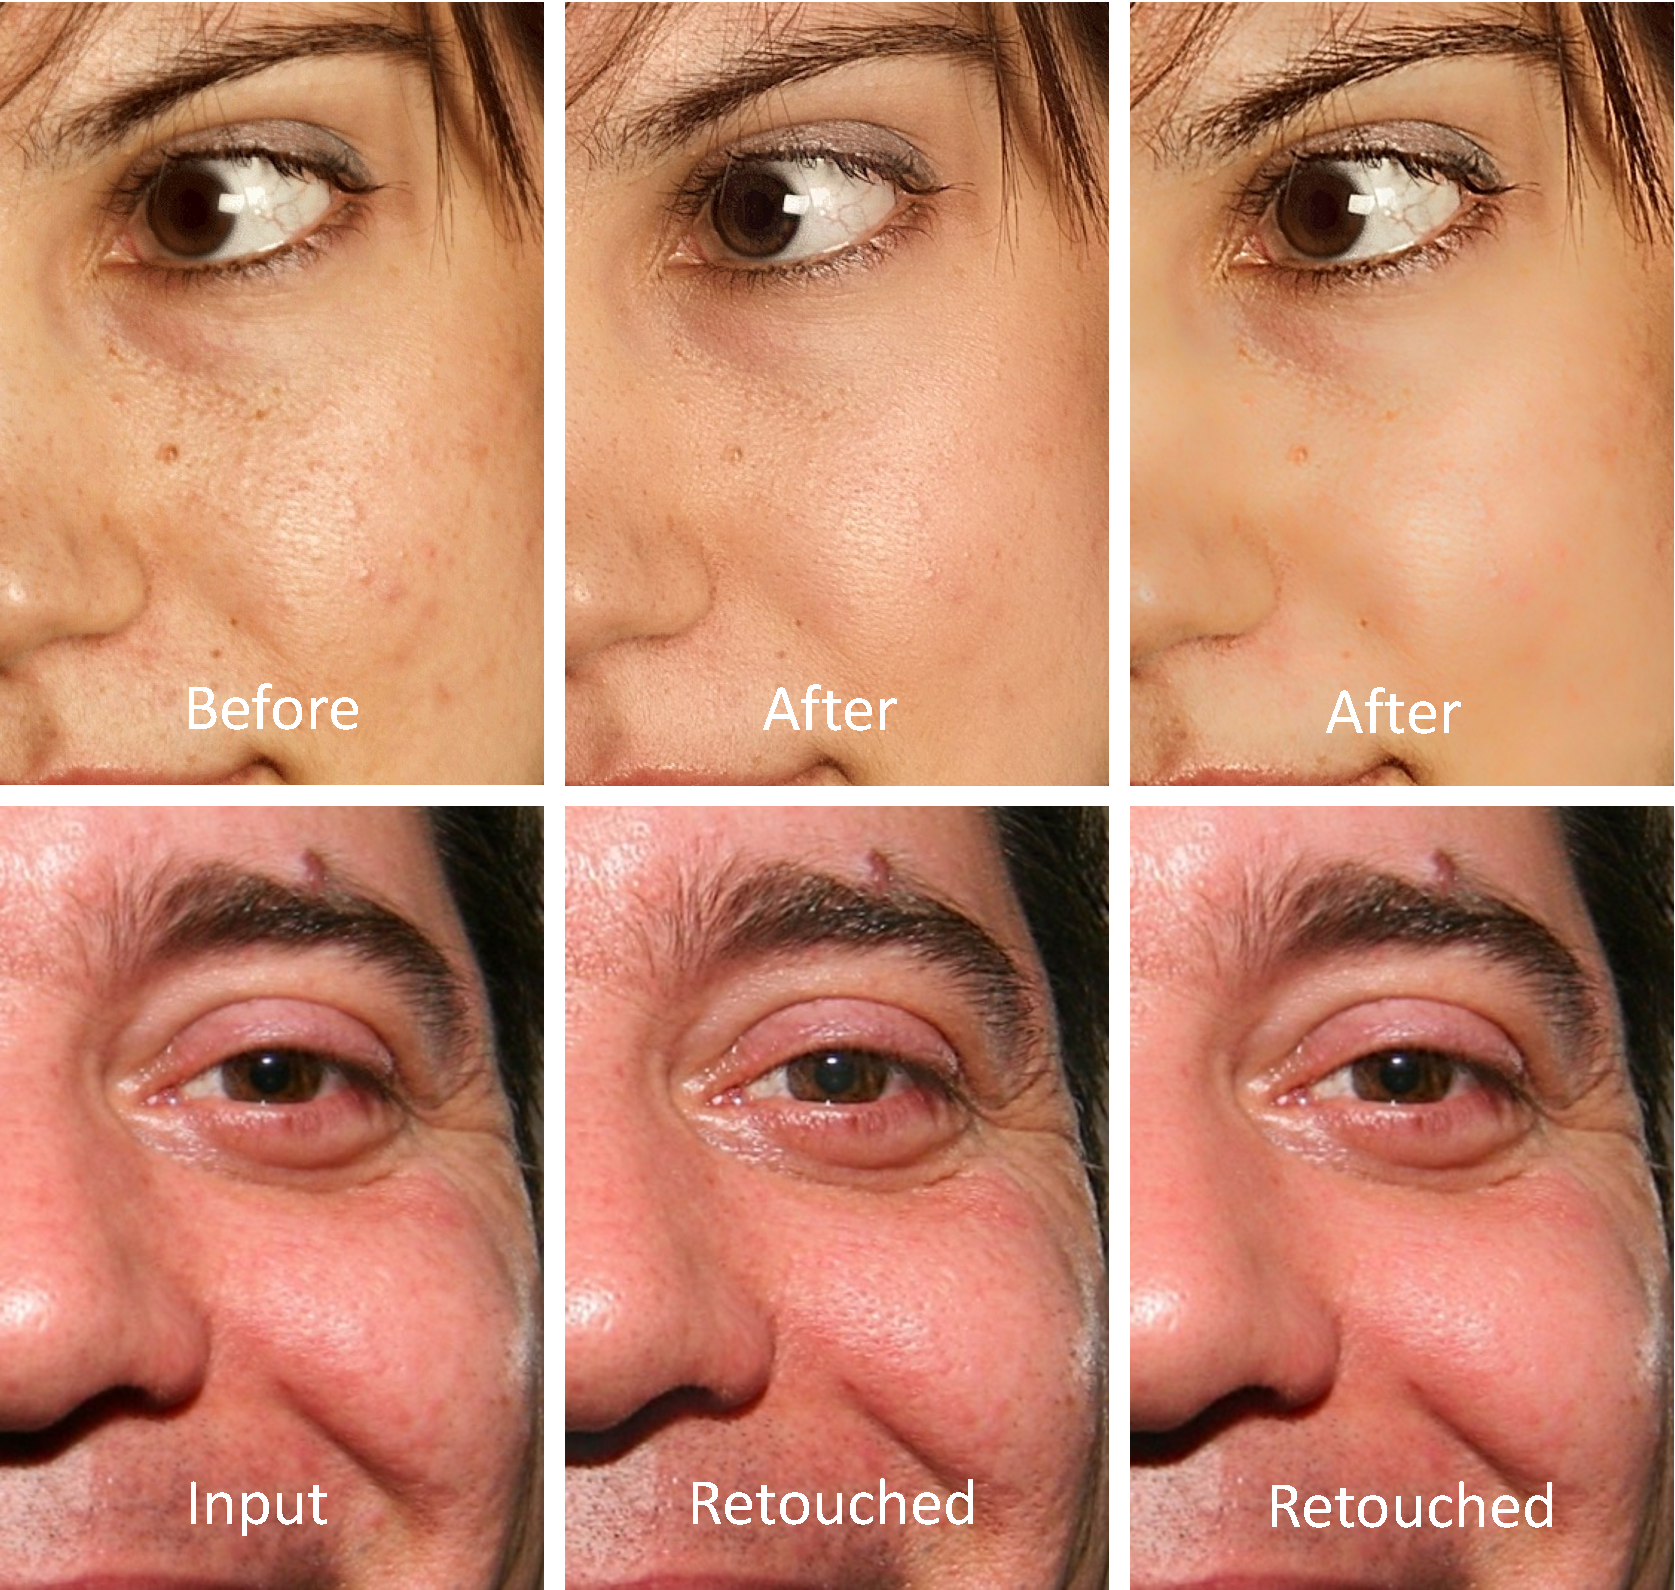
\includegraphics[width=0.8\columnwidth]{Chapters/detail-retouching-figs/Nuances.pdf}
  % \hfill
    \caption{Our patch-adaptive technique can accurately capture the nuances between different
    retouching styles as given by the examples (top row).}
\label{fig:retouchingstyles}
\end{figure}

In all experiments, intricate details of the desired retouching, such as small-scale texture, eye, facial hair or material details, and global features, such as overall lighting and tone, are accurately reproduced. It is interesting to observe that the \emph{glamour} implied by, e.g., the example retouching in Figure~\ref{fig:newdataset_ex} is transferred from the example pair very accurately without causing an artificial look. Zooming into the skin reveals that pores and wrinkles are minimised, and the blemishes and discolouring of the skin are eliminated. At the same time, depending on the retouching edit, details, such as eyes or material texture, are more highlighted or preserved, and delicate features such as hair are preserved well (Figures ~\ref{fig:newdataset_ex}, ~\ref{fig:material_res} and ~\ref{fig:retouchingstyles}). 


In summary, the proposed technique efficiently edits such intricate details, due to the significantly distinct local statistics of the texture at multiple scales, without affecting overlaying structures thanks to its spatially-varying nature and frequency decomposition. 

\subsection{Comparison with the state-of-the-art}
\label{sec:Comparisons}


Although there are various works related to automatic photo enhancement, to the best of our knowledge, none of them works with a single example pair for detail retouching. Therefore, I compare the results with closely related automatic image-to-image translation methods, namely U-Net \cite{ronneberger2015u}, ASAPNet generator \cite{shaham2021spatially}, and Deep edge-aware filters \cite{xu2015deep}. 

I trained each network from scratch with one \textit{before-after} pair. To train the U-Net architecture, I changed the activation function of its last layer to ReLU and used $l_1$ loss function with Adam optimiser (same as ours). Similar to the proposed method, ASAPNet is also a spatially-adaptive network. However, it is instead designed to hallucinate new details. Therefore, I trained their generator model in a similar fashion with $l1$ loss, removing the discriminator. After observing that bilinear downsampling in their model causes checkerboard artifacts, I removed this operator and learned an MLP per pixel, which caused the model to be highly complex with too many parameters. 


\begin{table*}[th]
\centering
\caption{Quantitative performance comparison for the reproduction of various image processing filters. Average PSNR and SSIM values are computed over 182 images of different types of images including faces, landscapes, materials, and rooms. Qualitative results can be found in the supplementary material.We highlight \colorbox{blue!25}{best PSNR} and \colorbox{orange!25}{best SSIM} results.}


\resizebox{\textwidth}{!}{\begin{tabular}{l@{\hskip 0.2in}c@{\hskip 0.1in}c@{\hskip 0.1in}c@{\hskip 0.1in}@{\hskip 0.1in}c@{\hskip 0.1in}c@{\hskip 0.1in}c}
    % \begin{tabular}{@{}cccccc@{}}
    \toprule
     \multicolumn{5}{c}{{Comparison results (PSNR in dB / SSIM)}} \\ \cline{1-5}
     {Filter Type} & {ASAPNet Generator} & {Deep Edge-aware} & {UNet} & {Ours}\\
     \midrule
    Gaussian & \cellcolor{orange!25}{39.36 / 0.983} & 36.52 / 0.979 & 40.52 / 0.979 & \cellcolor{blue!25}{40.67 / 0.983} \\%\midrule
    %   \hline
     Unsharp Mask & 29.77 / 0.889 & 32.62 / \cellcolor{orange!25}{0.959} & 32.05 / 0.919 & \cellcolor{blue!25}{33.88 /
0.931}\\%\midrule
    %   \hline
     Bilateral Filter & 33.65 / 0.936 & 33.56 / 0.958 & 34.00 / 0.939 & \colorbox{blue!25}{38.16 / 0.965}\\%\midrule
    %   \hline
     Local Laplacian ($\alpha=2$, $\sigma =0.2$) & 30.85 / 0.913 & 30.69 / 0.943 & 31.53 / 0.925 & \cellcolor{blue!25}{33.50 / 0.950} \\%\midrule
    %   \hline
     Local Laplacian ($\alpha=0.5$, $\sigma =0.1$) & 31.98 / 0.909 & 31.62 / 0.931 & 33.08 / 0.929 & \cellcolor{blue!25}{35.72 / 0.940}

     \\\bottomrule
    %  \hline
    \end{tabular}}
\label{tablecomparison}
\end{table*}


% These results are included in Table 1 for the filter types indicated in rows. The training strategy for the state-of-the-art methods is summarised in Section \ref{sec:Comparisons}. Before-after pairs along with additional results can be found in the supplementary material. Image courtesy of Arnaud Rougetet (landscape) and virtualhorizonstudio (alarm clock). (CC-BY and PixelSquid)


For a fair comparison with contemporary methods, I trained each network with the same example pair processed by four algorithmic filters: Gaussian, unsharp masking, Bilateral, and local Laplacian filters (LLF). As LLFs can perform a wide range of edge-aware operations, I apply two different versions of the filter, one for smoothing ($\alpha=2,  \sigma=0.2$) and one for enhancing details ($\alpha=0.5, \sigma=0.1$). Each network is trained from scratch with the same example pair resized to $256 \times 256$ for the corresponding filter. 
%($\alpha=0.7, \sigma=0.4$)
%Itested the models with 100 face images, randomly sampled from MIT-Adobe FiveK \cite{Bychkovsky11Learning}, 
To prove the generalisability of the technique, I tested the models on different types of images, namely face images (100 images that are randomly sampled from MIT-Adobe FiveK \cite{Bychkovsky11Learning}), material images (22 images), room images (30), and landscape images (30). Each type was trained separately with its corresponding example pair. For instance, I trained an example pair of landscape images to test the model on landscape images. I evaluated the models using average PSNR and SSIM values. To generate the ground truths of the input images, I applied the same filter as applied to the before example image to obtain the after image. I trained each model in Y-channel after converting RGB images to their YCbCr versions and evaluated the results for Y-channel images. I duplicated the Y-channel in case the model requires three-channel images. 


To obtain the UNet results for each type of images, I ran an additional experiment in which I changed the number of trainable parameters by removing some layers and trained the network from scratch for unsharp masking and bilateral filtering. The number of chosen parameters were 0.1M (with a few convolutional layers), 1.8M, 10M and 30M. For material images, I observed that 10M performed the best in terms of PSNR and SSIM values, while for other types of images 30M performed best. I tested the trained models on the images of the corresponding types and computed average PSNR values. Later, I chose the model with the best-performing parameters for each type of image for the quantitative comparison (Table \ref{tablecomparison}).

Overall, our method can outperform all architectures for each considered filter in terms of PSNR values. UNet shows the closest performance, but their network capacity is significantly higher than the proposed framework (0.16M). As the filter becomes more complex, the performance gap increases. For instance, other methods perform fairly well in simple algorithmic filters, such as Gaussian or unsharp masking. However, in spatially-varying filters, namely Bilateral filter or LLFs, this method proves more generalisable thanks to its path-adaptive structure. 

Figures \ref{fig:QualitativeComp_BF}, \ref{fig:QualitativeComp_LLF_a2}, and \ref{fig:QualitativeComp_LLF_a05} further demonstrates that our technique can preserve and edit intricate details, such as text, texture, or leaves, more effectively without causing much distortion. The nonlinear bilateral filter and Local Laplacian filters pose an additional challenge, especially in a one-shot setting. However, the proposed approach can still perform edge-aware filtering with higher accuracy than the baselines. Note that these examples are selected from the results I obtained for the quantitative comparison (Table \ref{tablecomparison}), where I only used the luminance channels and downsampled the images to $256 \times 256$. 



\begin{figure*}%[th]%[tph]{
  \centering
      
\includegraphics[width=.82\linewidth]{Chapters/detail-retouching-figs/One-shot-labels.pdf}

  \includegraphics[width=\linewidth]{Chapters/detail-retouching-figs/Qualitative_zoomed_BF.pdf}
    \caption{Qualitative comparison with baseline approaches on bilateral filtering. Bilateral filter is a nonlinear filter designed for smoothing the surfaces while preserving the edges. Results show that our proposed technique captures the bilateral-filtering effect more effectively, reducing the roughness of the surfaces while maintaining important details.} 

   \label{fig:QualitativeComp_BF}%
\end{figure*}

    
 %   These results are included in Table 1 for the filter types indicated in rows. The training strategy for the state-of-the-art methods is summarised in Section \ref{sec:Comparisons}. Before-after pairs along with additional results can be found in the supplementary material. Image courtesy of Arnaud Rougetet (landscape) and virtualhorizonstudio (alarm clock). (CC-BY and PixelSquid).

\begin{figure*}%[th]%[tph]{
  \centering
      
\includegraphics[width=.82\linewidth]{Chapters/detail-retouching-figs/One-shot-labels.pdf}
  \includegraphics[width=\linewidth]{Chapters/detail-retouching-figs/Qualitative_zoomed_LLF_a2_s02.pdf}
    \caption{Qualitative comparison with baseline approaches on Local Laplacian filter (LLF) ($\alpha=2, \sigma=0.2$). LLF is another edge-aware nonlinear filter designed for multiple tasks, namely edge-preserving smoothing, detail enhancement, tone mapping, and inverse tone mapping. In these examples, the parameters are chosen to have an edge-preserving smoothing effect, similar to bilateral filtering. Results show that ours offer smoother textures.} 

   \label{fig:QualitativeComp_LLF_a2}%
\end{figure*}

%These results are included in Table 1 for the filter types indicated in rows. The training strategy for the state-of-the-art methods is summarised in Section \ref{sec:Comparisons}. Before-after pairs along with additional results can be found in the supplementary material. Image courtesy of Arnaud Rougetet (landscape) and virtualhorizonstudio (alarm clock). (CC-BY and PixelSquid).

\begin{figure*}%[th]%[tph]{
  \centering
    
\includegraphics[width=.82\linewidth]{Chapters/detail-retouching-figs/One-shot-labels.pdf}
  \includegraphics[width=\linewidth]{Chapters/detail-retouching-figs/Qualitative_zoomed_LLF_a05_s01.pdf}
    \caption{Qualitative comparison with baseline approaches on Local Laplacian filter (LLF) ($\alpha=0.5, \sigma=0.1$). Here, the parameters are chosen accordingly to enhance the details. Our results highlight edges, such as the transition between the cloud and the sky, the numbers in the clock or the texture on the bed sheet.} 

   \label{fig:QualitativeComp_LLF_a05}%
\end{figure*}

\newpage
\subsection{Limitations and Future Work}
\begin{figure}[th] % "[t!]" placement specifier just for this example
	\centering
	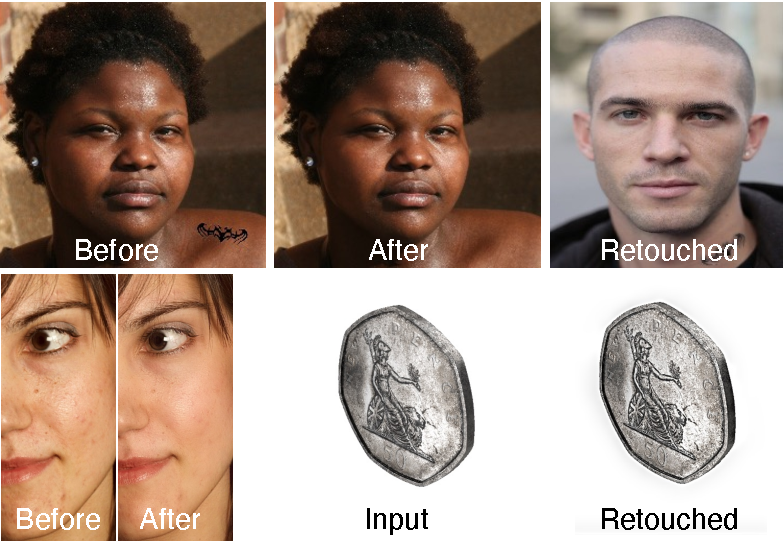
\includegraphics[width=0.8\columnwidth]{Chapters/detail-retouching-figs/Limitations.pdf}
    \caption{\label{fig:limitations} The proposed technique cannot accurately handle extreme non-repeating local effects such as tattoos (top), and when example and input images are of very different semantics (bottom). Image courtesy of bgaj23 (coin). (PixelSquid).}

\end{figure}
A primary limitation of this work is its dependence on local patches at different scales, disregarding their spatial location. Hence, the method is most useful when details are retouched based on local and repeated characteristics of an image. Non-repeating spatially-dependent strong effects, e.g., tattoos or portrait stylisations with spatially varying lighting~\cite{Shih14Style}, cannot be handled by the current technique (see Figure \ref{fig:limitations}).


Since the method relies on a single example image pair, transferring filters applied to arbitrary images~\cite{Yan14Automatic} is out of the scope of this work. Example and input images are required to have similar semantics for predictable transfer. Extending the technique to more than one pair of example images will require us to have consistently retouched details on all those example images. Finally, the example before and after images are required to be perfectly aligned. This requirement can be alleviated by incorporating an ICP~\cite{Besl92AMethod}-like approach into the optimisation in Section~\ref{sec:Methodology}. 

Although the main focus in this paper is learning artist-driven subjective retouching edits, the proposed technique is general. It can be extended to transfer arbitrary image transformations, significantly where details are modified. Thus, I plan to investigate the technique further as a general transfer method for image-to-image translation. The patch-adaptive nature of the mappings makes them amenable to analysis.
